\section{Własności miary Lebesgue'a w $\Rn$}

Konstrukcja zbioru Vitalego pokazała, gdzie leży nieprzekraczalna granica teorii: nie da się zmierzyć wszystkich podzbiorów $\mathbb{R}^n$ w sposób przeliczalnie addytywny i niezmienniczy na translacje. Wiemy już dokładnie, jak wygląda dziedzina miary Lebesgue’a $\mathcal{L}(\mathbb{R}^n)$. Pora zatem zapytać o cechy samej miary: na ile zdefiniowana funkcja $\lambda^n$ jest wyjątkowa? Czy istnieją inne miary spełniające te same postulaty geometryczne? W niniejszym rozdziale wykażemy twierdzenie o jednoznaczności miary Lebesgue'a oraz zbadamy jej zachowanie przy izometriach, przekształceniach liniowych i w operacjach algebraicznych (twierdzenie Steinhausa).

\subsection{Jednoznaczność miary Lebesgue'a}

Podstawowym pytaniem teorii miary jest to, na ile aksjomy objętości oraz postulaty geometryczne determinują miarę Lebesgue'a. Poniższe twierdzenia pokazują, że miara ta jest wyznaczona jednoznacznie zarówno przez geometrię kostek, jak i przez strukturę algebraiczną grupy $(\Rn, +)$.

\begin{tw}[Jednoznaczność przez objętość kostek]\label{tw:jednoznacznosc_kostki}
    Niech $\mu$ będzie miarą określoną na $\sigma$-algebrze $\Leb{\Rn}$ taką, że dla każdej kostki domkniętej $P \subset \Rn$ zachodzi:
    \begin{equation}
        \mu(P) = V^n(P).
    \end{equation}
    Wówczas $\mu = \lambda^n$ na całej $\sigma$-algebrze $\Leb{\Rn}$.
\end{tw}

\begin{dow}
    Niech $A \in \Leb{\Rn}$ oraz niech $\{P_j\}_{j=1}^\infty$ będzie dowolnym ciągiem kostek domkniętych pokrywającym $A$, tj. $A \subset \bigcup_{j=1}^\infty P_j$. Z przeliczalnej podaddytywności miary $\mu$:
    \begin{equation*}
        \mu(A) \le \mu\left(\bigcup_{j=1}^\infty P_j\right) \le \sum_{j=1}^\infty \mu(P_j) = \sum_{j=1}^\infty V^n(P_j).
    \end{equation*}
    Przechodząc do infimum po wszystkich przeliczalnych pokryciach kostkami domkniętymi, otrzymujemy bezpośrednio:
    \begin{equation*}
        \mu(A) \le \lambda^{*n}(A) = \lambda^n(A).
    \end{equation*}

    Aby dowieść nierówności przeciwnej, załóżmy najpierw, że zbiór $A \in \Leb{\Rn}$ jest ograniczony. Wówczas istnieje duża kostka domknięta $P \supset A$. Zbiór $P \setminus A$ jest mierzalny, więc z pierwszej części dowodu:
    \begin{equation*}
        \mu(P \setminus A) \le \lambda^n(P \setminus A) < +\infty.
    \end{equation*}
    Korzystając ze skończonej addytywności miar na zbiorach o skończonej mierze:
    \begin{equation*}
        \mu(P) - \mu(A) \le \lambda^n(P) - \lambda^n(A).
    \end{equation*}
    Ponieważ z założenia $\mu(P) = V^n(P) = \lambda^n(P) < +\infty$, odejmując tę wartość obustronnie, uzyskujemy:
    \begin{equation*}
        \lambda^n(A) \le \mu(A),
    \end{equation*}
    co daje $\mu(A) = \lambda^n(A)$ dla wszystkich zbiorów ograniczonych.

    Gdy $A$ jest zbiorem nieograniczonym, definiujemy ciąg warstw rozłącznych:
    \begin{equation*}
        A_1 = A \cap [-1, 1]^n, \quad A_j = A \cap \left( [-j, j]^n \setminus [-(j-1), j-1]^n \right) \quad \text{dla } j \ge 2.
    \end{equation*}
    Zbiory $A_j$ są ograniczone, mierzalne i parami rozłączne, a ponadto $A = \bigcup_{j=1}^\infty A_j$. Z przeliczalnej addytywności obu miar:
    \begin{equation*}
        \mu(A) = \sum_{j=1}^\infty \mu(A_j) = \sum_{j=1}^\infty \lambda^n(A_j) = \lambda^n(A),
    \end{equation*}
    co kończy dowód.
\end{dow}


\begin{tw}[Jedyność miary Haara w $\Rn$]\label{tw:jednoznacznosc_haara}
    Niech $\mu$ będzie miarą borelowską w $\Rn$ spełniającą dwa warunki:
    \begin{enumerate}
        \item[(i)]
              \textbf{niezmienniczość na translacje}: $\forall A \in \BorelRn, \forall x \in \Rn \colon \quad \mu(x + A) = \mu(A)$;
        \item[(ii)] \textbf{normalizacja na kostce jednostkowej}: $\mu([0, 1)^n) = 1$. \end{enumerate}
    Wówczas $\mu = \lambda^n$ na $\sigma$-algebrze zbiorów borelowskich $\BorelRn$.
\end{tw}
\begin{dow}
    Niech $P_0 = [0, 1)^n$. Dla dowolnej liczby naturalnej $k \wlr 1$ podzielmy każdy z boków kostki $P_0$ na $k$ równych przedziałów postaci $[\frac{i-1}{k}, \frac{i}{k})$.
    Otrzymujemy w ten sposób podział $P_0$ na $k^n$ rozłącznych kostek o krawędzi $\frac{1}{k}$.
    Każda z tych kostek jest translacją kostki $Q_k = [0, \frac{1}{k})^n$.
    Z addytywności i translacyjnej niezmienniczości miary $\mu$:
    \begin{equation*}
        1 = \mu(P_0) = \sum_{j=1}^{k^n} \mu(Q_k) = k^n \mu(Q_k) \implies \mu(Q_k) = \frac{1}{k^n} = \lambda^n(Q_k).
    \end{equation*}
    Dowolną kostkę o krawędziach wymiernych $\prod_{i=1}^n [a_i, b_i)$ (gdzie $a_i = \frac{p_i}{k}, b_i = \frac{q_i}{k}$) można złożyć ze skończonej liczby rozłącznych kostek przystających do $Q_k$. Stąd $\mu(P) = \lambda^n(P)$ dla każdej kostki o wierzchołkach wymiernych. Ponieważ rodzina takich kostek tworzy $\pi$-układ generujący topologię euklidesową oraz $\sigma$-algebrę borelowską $\BorelRn$, a miary są $\sigma$-skończone (przykryte ciągiem $[-m, m)^n$), z twierdzenia o jednoznaczności rozszerzenia miary na $\pi$-układach (lemat Dynkina o klasie monotonicznej) wynika, że $\mu(B) = \lambda^n(B)$ dla każdego $B \in \BorelRn$.
\end{dow}



\subsection{Własności geometryczne: izometrie i przekształcenia liniowe}

\begin{figure}[htbp]
    \centering
    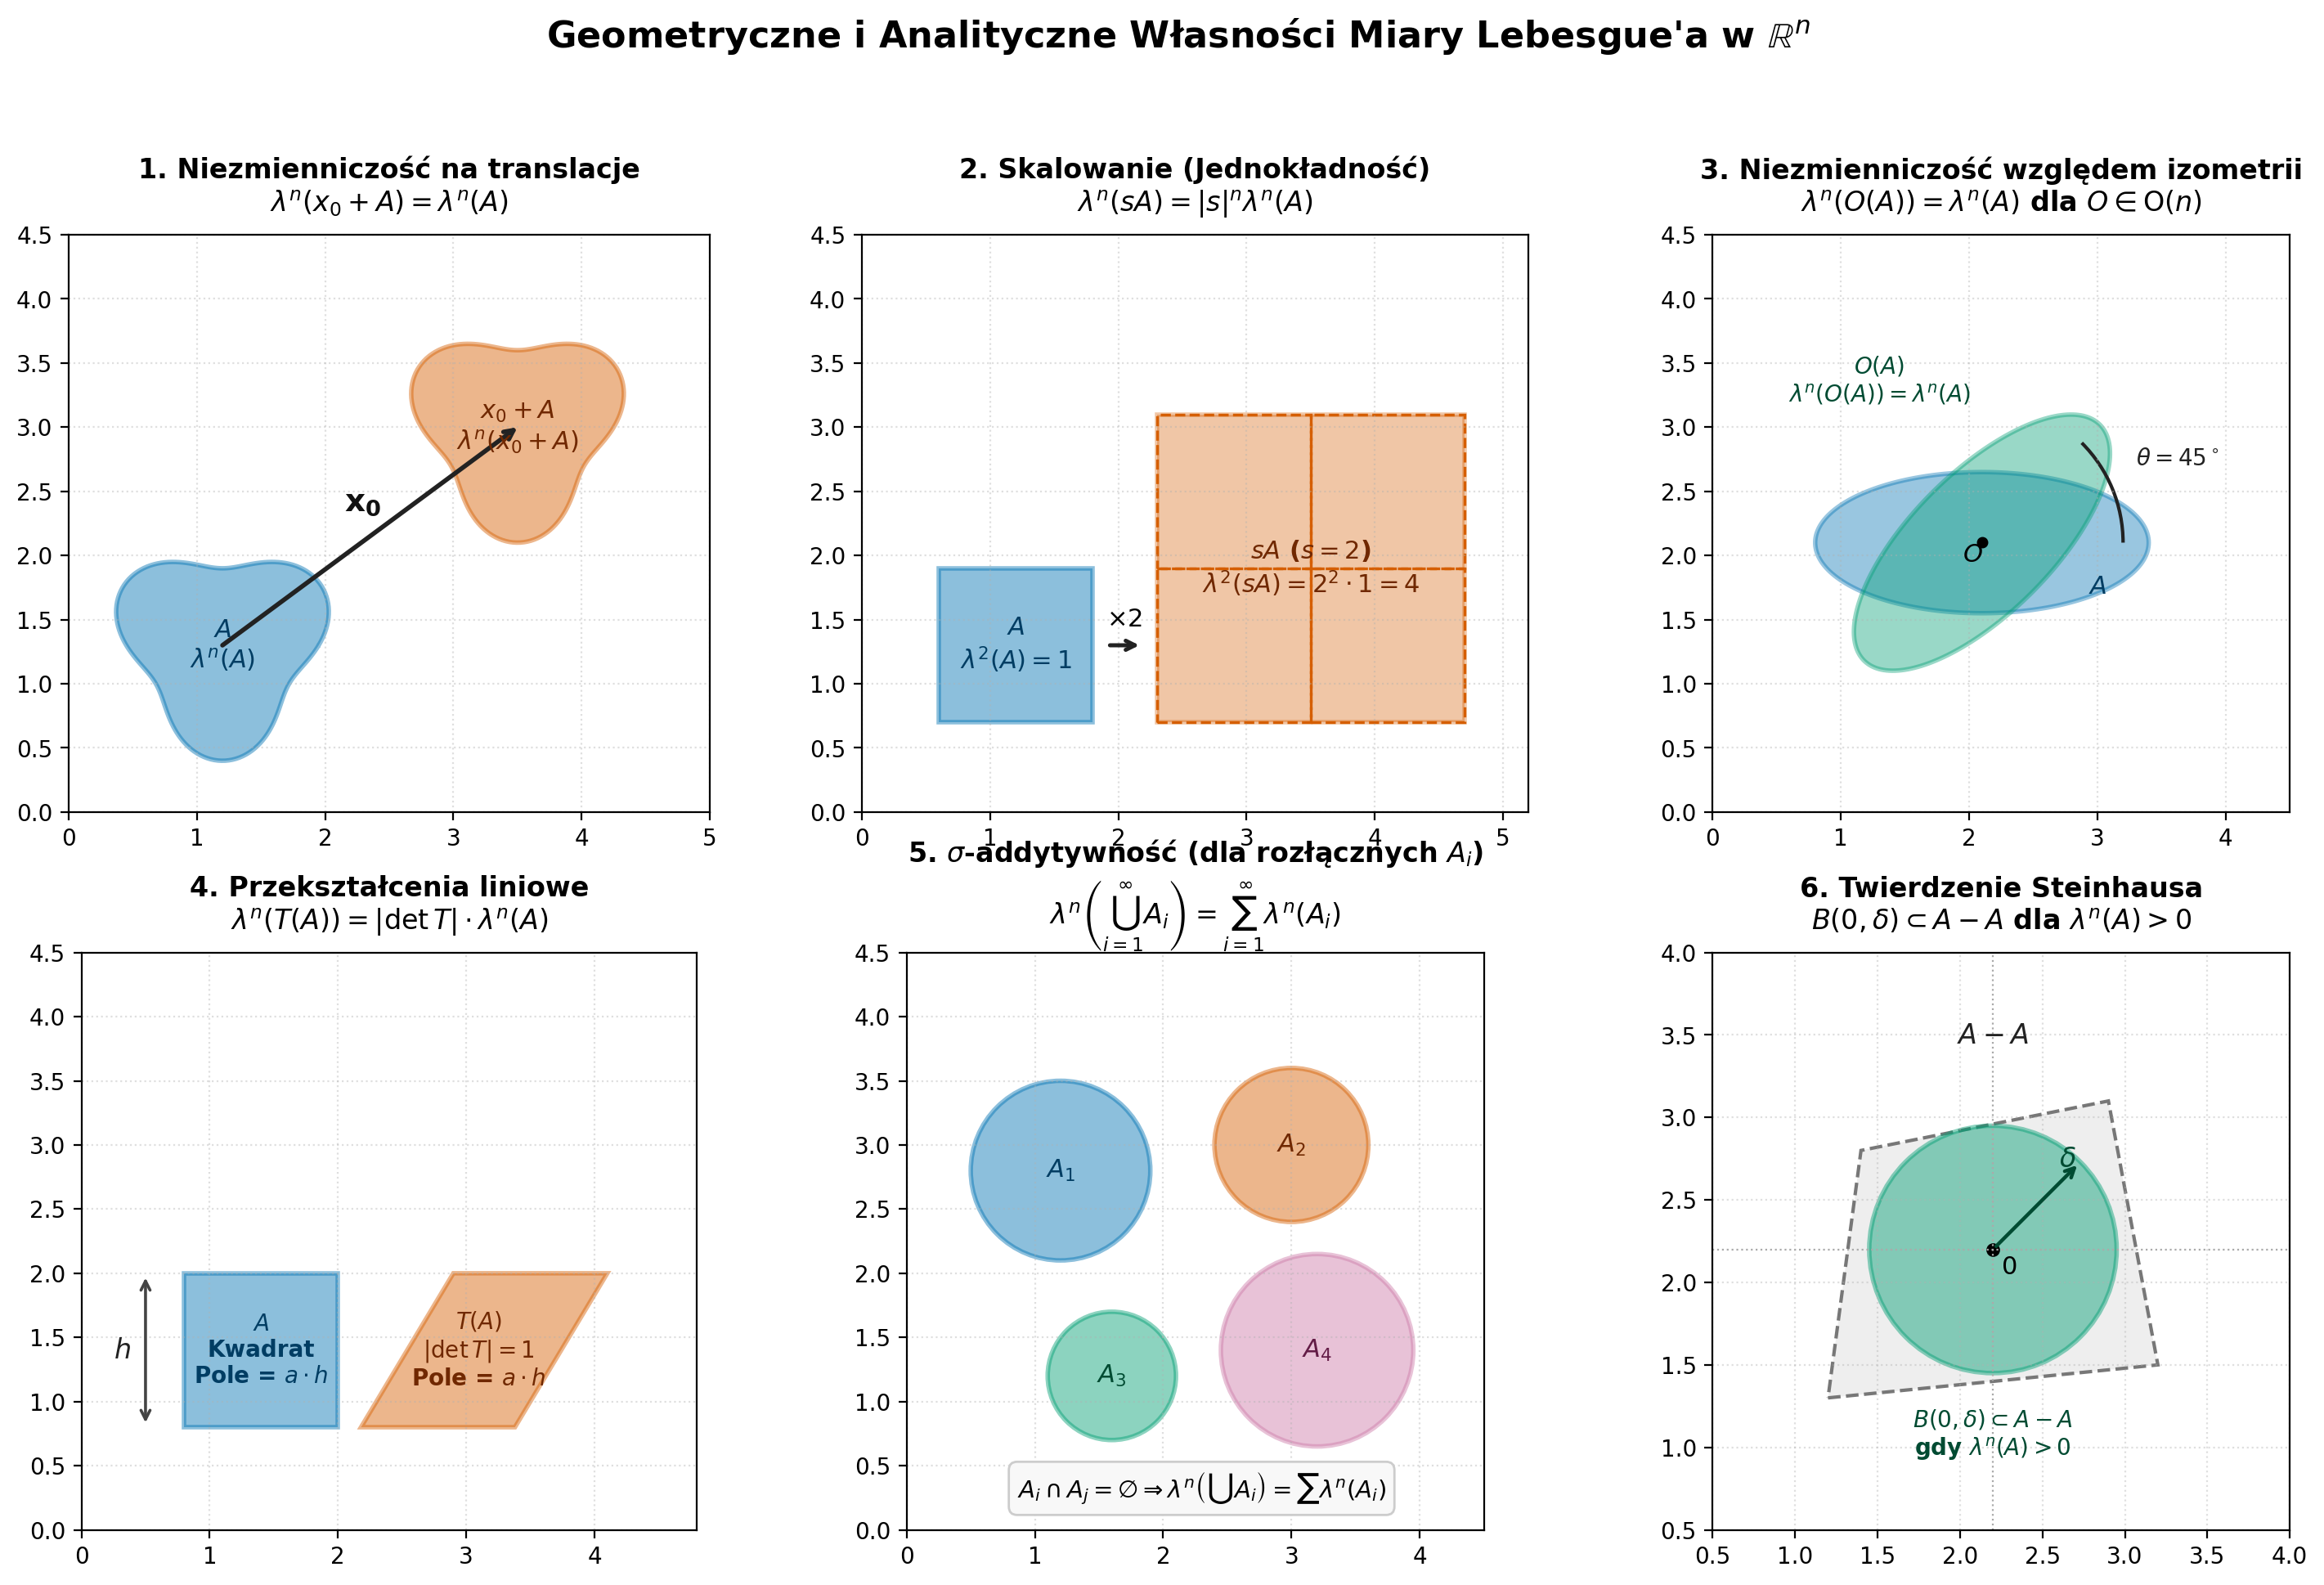
\includegraphics[width=0.95\textwidth]{wlasnosci_miary_lebesguea.png}
    \caption{Geometryczna interpretacja kluczowych własności miary Lebesgue'a w $\Rn$: translacji, skalowania, izometrii, przekształceń liniowych, $\sigma$-addytywności oraz twierdzenia Steinhausa.}
    \label{fig:wlasnosci_miary}
\end{figure}

\begin{tw}[Zachowanie miary przy translacji i skalowaniu]
    Niech $A \in \Leb{\Rn}$, $x_0 \in \Rn$ oraz $s \in \mathbb{R}$. Wówczas:
    \begin{enumerate}
        \item $x_0 + A \in \Leb{\Rn}$ oraz $\lambda^n(x_0 + A) = \lambda^n(A)$;
        \item $sA \in \Leb{\Rn}$ oraz $\lambda^n(sA) = |s|^n \lambda^n(A)$.
    \end{enumerate}
\end{tw}

\begin{tw}[Przekształcenia liniowe]\label{tw:transformacja_liniowa}
    Niech $T \colon \Rn \to \Rn$ będzie operatorem liniowym reprezentowanym przez macierz $M \in M_{n \times n}(\mathbb{R})$. Jeżeli $A \in \Leb{\Rn}$, to $T(A) \in \Leb{\Rn}$ oraz:
    \begin{equation}
        \lambda^n(T(A)) = |\det T| \cdot \lambda^n(A).
    \end{equation}
\end{tw}

\begin{dow}
    Rozpatrzmy dwa przypadki w zależności od rzędu macierzy przekształcenia:

    \paragraph{Przypadek 1: $\det T = 0$.}
    Gdy operator $T$ jest osobliwy, obraz $T(\Rn)$ jest podprzestrzenią liniową wymiaru $k < n$. Podprzestrzeń właściwa w $\Rn$ po odpowiednim obrocie zawiera się w hiperpłaszczyźnie $\{x \in \Rn \colon x_n = 0\}$, która ma miarę Lebesgue'a zero ($\lambda^n = 0$). Ponieważ $T(A) \subset T(\Rn)$, z zupełności miary wynika, że $T(A) \in \Leb{\Rn}$ oraz $\lambda^n(T(A)) = 0 = |\det T| \lambda^n(A)$.

    \paragraph{Przypadek 2: $\det T \neq 0$.}
    Gdy $T$ jest izomorfizmem, z twierdzeń algebry liniowej wynika, że macierz $T$ można rozłożyć na iloczyn skończenie wielu macierzy elementarnych odpowiadających operacjom:
    \begin{enumerate}
        \item[(a)] pomnożeniu jednej współrzędnej przez skalar $c \neq 0$ (wtedy $\det E_1 = c$ oraz objętość kostki skaluje się o $|c|$);
        \item[(b)] dodaniu do jednej współrzędnej krotności innej współrzędnej (tzw. ścinanie; wówczas $\det E_2 = 1$, a na mocy zasady Cavalieriego miara prostopadłościanu nie ulega zmianie);
        \item[(c)] permutacji osi współrzędnych ($\det E_3 = \pm 1$, miara kostki pozostaje niezmiennicza).
    \end{enumerate}
    Zatem dla każdej macierzy elementarnej $E$ oraz kostki $P$ zachodzi $\lambda^n(E(P)) = |\det E| V^n(P)$. Definiując miarę $\mu(B) := \lambda^n(T(B))$ na $\Borel{\Rn}$, zauważamy, że $\mu$ jest miarą translacyjnie niezmienniczą. Na mocy Twierdzenia \ref{tw:jednoznacznosc_haara} zachodzi tożsamość $\mu(B) = \mu([0, 1)^n) \lambda^n(B) = |\det T| \lambda^n(B)$.
    Przejście z $\Borel{\Rn}$ na $\Leb{\Rn}$ wynika natychmiast z faktu, że $T$ jako homeomorfizm zachowuje zbiory miary zero (zbiory pomijalne).
\end{dow}

\begin{wn}[Niezmienniczość względem izometrii]
    Każda izometria przestrzeni euklidesowej $\Phi \colon \Rn \to \Rn$ ma postać $\Phi(x) = Ox + x_0$, gdzie $O \in \mathrm{O}(n)$ jest macierzą ortogonalną ($O^T O = I$), a $x_0 \in \Rn$. Ponieważ $\det O = \pm 1$, dla każdego zbioru $A \in \Leb{\Rn}$ zachodzi:
    \begin{equation}
        \lambda^n(\Phi(A)) = |\det O| \cdot \lambda^n(A) = \lambda^n(A).
    \end{equation}
    W szczególności miara Lebesgue'a jest niezmiennicza na obroty wokół środka układu współrzędnych oraz symetrie zwierciadlane.
\end{wn}

\subsection{Własności strukturalne: bezatomowość i własność Darboux}

\begin{defi}[Atom miary]
    Niech $(X, \mathcal{M}, \mu)$ będzie przestrzenią z miarą. Zbiór $A \in \mathcal{M}$ o mierze $\mu(A) > 0$ nazywamy \textbf{atomem miary} $\mu$, jeżeli dla każdego podzbioru mierzalnego $B \in \mathcal{M}, B \subset A$ zachodzi:
    \begin{equation}
        \mu(B) = 0 \quad \text{albo} \quad \mu(B) = \mu(A).
    \end{equation}
    Miarę $\mu$ nazywamy \textbf{bezatomową}, jeżeli nie posiada ona żadnych atomów.
\end{defi}

\begin{tw}[Bezatomowość miary Lebesgue'a]
    Miara Lebesgue'a $\lambda^n$ w $\Rn$ jest miarą bezatomową.
\end{tw}

\begin{dow}
    Niech $A \in \Leb{\Rn}$ spełnia $\lambda^n(A) > 0$. Rozważmy hiperpłaszczyzny prostopadłe do pierwszej osi współrzędnych: $H_t = \{x \in \Rn \colon x_1 \le t\}$ dla $t \in \mathbb{R}$. Zdefiniujmy funkcję przekroju:
    \begin{equation*}
        f(t) := \lambda^n(A \cap H_t).
    \end{equation*}
    Funkcja $f$ jest niemalejąca, $\lim_{t \to -\infty} f(t) = 0$ oraz $\lim_{t \to +\infty} f(t) = \lambda^n(A)$. Ponadto $f$ jest ciągła, gdyż dla dowolnych $t_1 < t_2$:
    \begin{equation*}
        0 \le f(t_2) - f(t_1) = \lambda^n(A \cap \{x \colon t_1 < x_1 \le t_2\}) \le \lambda^n([t_1, t_2] \times \mathbb{R}^{n-1} \cap A).
    \end{equation*}
    Z własności Darboux dla funkcji ciągłej $f$ istnieje punkt $t_0 \in \mathbb{R}$ taki, że:
    \begin{equation*}
        f(t_0) = \lambda^n(A \cap H_{t_0}) = \frac{1}{2} \lambda^n(A).
    \end{equation*}
    Kładąc $B = A \cap H_{t_0}$, otrzymujemy podzbiór mierzalny $B \subset A$ o mierze ściśle pośredniej: $0 < \lambda^n(B) < \lambda^n(A)$. Zbiór $A$ nie jest więc atomem, co dowodzi bezatomowości miary $\lambda^n$.
\end{dow}

\begin{wn}[Własność Darboux dla miary Lebesgue'a]
    Dla każdego zbioru mierzalnego $A \in \Leb{\Rn}$ oraz dowolnej liczby rzeczywistej $c$ spełniającej $0 \le c \le \lambda^n(A)$ istnieje zbiór mierzalny $B \subset A$ taki, że:
    \begin{equation}
        \lambda^n(B) = c.
    \end{equation}
\end{wn}

\subsection{Twierdzenie Steinhausa}

Znakomitą ilustracją głębokiego powiązania struktury miarowej Lebesgue'a ze strukturą algebraiczną i topologiczną $\Rn$ jest twierdzenie udowodnione przez Hugona Steinhausa w 1920 roku. Pokazuje ono, że zbiór dodatniej miary Lebesgue'a — chociaż może być nigdziegęsty — generuje zbiór różnic o niepustym wnętrzu.

\begin{defi}[Zbiór różnic]
    Dla dowolnego podzbioru $A \subset \Rn$ jego \textbf{zbiorem różnic} nazywamy zbiór:
    \begin{equation}
        A - A := \{x - y \colon x, y \in A\}.
    \end{equation}
\end{defi}

\begin{tw}[Twierdzenie Steinhausa]\label{tw:steinhaus}
    Jeżeli zbiór $A \in \Leb{\Rn}$ ma dodatnią miarę Lebesgue'a ($\lambda^n(A) > 0$), to zbiór różnic $A - A$ zawiera otwartą kulę o środku w zerze, to znaczy:
    \begin{equation}
        \exists \, \delta > 0 \quad \text{taki, że} \quad B(0, \delta) \subset A - A.
    \end{equation}
\end{tw}

\begin{dow}
    Z regularności miary Lebesgue'a możemy bez zmniejszenia ogólności założyć, że $A$ jest zbiorem o skończonej mierze ($0 < \lambda^n(A) < +\infty$).

    Ustalmy $\varepsilon = \frac{1}{3} \lambda^n(A) > 0$. Na mocy Twierdzenia~\ref{tw:charakter_mierzalnosci} o aproksymacji istnieje zbiór otwarty $U \subset \Rn$ taki, że $A \subset U$ oraz:
    \begin{equation*}
        \lambda^n(U \setminus A) < \varepsilon.
    \end{equation*}
    Zbiór otwarty $U$ jest sumą przeliczalnej rodziny kostek otwartych. Wobec tego musi istnieć kostka otwarta $Q \subset U$ taka, że:
    \begin{equation*}
        \lambda^n(A \cap Q) > \frac{3}{4} \lambda^n(Q).
    \end{equation*}
    Niech $d$ oznacza długość krawędzi kostki $Q$. Wybierzmy $\delta > 0$ na tyle małe, aby dla każdego wektora przesunięcia $h \in \Rn$ o normie $\|h\| < \delta$ kostka przesunięta $Q + h$ w znacznym stopniu pokrywała się z $Q$, w szczególności spełniając:
    \begin{equation*}
        \lambda^n(Q \cap (Q + h)) > \frac{3}{4} \lambda^n(Q).
    \end{equation*}
    Dla każdego $h \in B(0, \delta)$ rozważmy przekrój $A \cap (A + h)$. Zauważmy, że zachodzi relacja teoriomnogościowa:
    \begin{equation*}
        (A \cap Q) \cup ((A + h) \cap (Q + h)) \subset Q \cup (Q + h).
    \end{equation*}
    Gdyby zbiory $A \cap Q$ oraz $(A + h) \cap (Q + h)$ były rozłączne, to suma ich miar nie mogłaby przekroczyć miary sumy kostek:
    \begin{align*}
        \lambda^n(Q \cup (Q + h)) & \ge \lambda^n(A \cap Q) + \lambda^n((A + h) \cap (Q + h))                                   \\
                                  & = \lambda^n(A \cap Q) + \lambda^n(A \cap Q) \quad \text{(z niezmienniczości translacyjnej)} \\
                                  & > \frac{3}{4} \lambda^n(Q) + \frac{3}{4} \lambda^n(Q) = \frac{3}{2} \lambda^n(Q).
    \end{align*}
    Z drugiej strony:
    \begin{equation*}
        \lambda^n(Q \cup (Q + h)) = \lambda^n(Q) + \lambda^n(Q + h) - \lambda^n(Q \cap (Q + h)) < 2\lambda^n(Q) - \frac{3}{4}\lambda^n(Q) = \frac{5}{4} \lambda^n(Q).
    \end{equation*}
    Otrzymana sprzeczność ($\frac{3}{2} \le \frac{5}{4}$) dowodzi, że zbiory $A$ oraz $A + h$ nie mogą być rozłączne:
    \begin{equation*}
        A \cap (A + h) \neq \emptyset \quad \text{dla każdego } h \in B(0, \delta).
    \end{equation*}
    Oznacza to, że dla każdego $h \in B(0, \delta)$ istnieją punkty $x, y \in A$ takie, że $x = y + h$, czyli $h = x - y \in A - A$. Stąd $B(0, \delta) \subset A - A$, co kończy dowód.
\end{dow}

\begin{uwaga}[Zastosowania twierdzenia Steinhausa]
    Twierdzenie Steinhausa dostarcza błyskawicznego, alternatywnego dowodu niemierzalności zbioru Vitalego $V \subset [0, 1] $ zdefiniowanego w Twierdzeniu~\ref{tw:vitali}:
    \begin{itemize}
        \item Gdyby zbiór Vitalego $V$ był mierzalny, to ponieważ $\bigcup_{k=1}^\infty (V + r_k) \supset [0, 1]$, musiałoby zachodzić $\lambda^1(V) > 0$.
        \item Z twierdzenia Steinhausa wynikałoby wówczas, że zbiór różnic $V - V$ zawiera pewien przedział $(-\delta, \delta)$.
        \item Jednak z konstrukcji zbioru Vitalego wynika, że różnica dwóch różnych elementów $v_1, v_2 \in V$ nigdy nie jest liczbą wymierną ($(V - V) \cap \mathbb{Q} = \{0\}$). Ponieważ w każdym przedziale $(-\delta, \delta)$ znajdują się niezerowe liczby wymierne, zbiór $V$ nie może zawierać żadnego takiego przedziału. Sprzeczność ta po raz kolejny dowodzi niemierzalności zbioru $V$.
    \end{itemize}
\end{uwaga}
